\documentclass[11pt,a4paper]{article}

% ---------- Packages ----------
\usepackage[utf8]{inputenc}
\usepackage[T1]{fontenc}
\usepackage[margin=1in]{geometry}
\usepackage{amsmath,amssymb}
\usepackage{booktabs}
\usepackage{longtable}
\usepackage{array}
\usepackage{graphicx}
\usepackage{tikz}
\usetikzlibrary{arrows.meta,positioning,shapes.geometric,fit,backgrounds}
\usepackage{enumitem}
\usepackage{xcolor}
\usepackage{hyperref}
\usepackage{fancyhdr}
\usepackage{titlesec}
\usepackage{tcolorbox}
\tcbuselibrary{skins,breakable}
\usepackage{parskip}
\usepackage{caption}

% ---------- Colors ----------
\definecolor{climoragreen}{HTML}{0B2E20}
\definecolor{climoraamber}{HTML}{FFB800}
\definecolor{climoralight}{HTML}{E8F5EC}

% ---------- Rupee symbol (NOT a built-in LaTeX command -- must be defined) ----------
\newcommand{\textrupee}{Rs.\,}

% ---------- Hyperref setup ----------
\hypersetup{
    colorlinks=true,
    linkcolor=climoragreen,
    citecolor=climoragreen,
    urlcolor=climoragreen,
    pdftitle={CLIMORA: Climate-aware Load Intelligence \& Moisture Optimization for Resource-efficient Air-conditioning},
    pdfauthor={Team CLIMORA -- Yuva Yodha Tech Hackathon 2026}
}

% ---------- Header/Footer ----------
\pagestyle{fancy}
\fancyhf{}
\fancyhead[L]{\small CLIMORA -- Technical Report}
\fancyhead[R]{\small Yuva Yodha Tech Hackathon 2026}
\fancyfoot[C]{\thepage}
\renewcommand{\headrulewidth}{0.4pt}

% ---------- Status label macros ----------
\newcommand{\validated}{\textcolor{climoragreen}{\textbf{[VALIDATED BY SOURCE]}}}
\newcommand{\design}{\textcolor{blue!60!black}{\textbf{[DESIGN DECISION]}}}
\newcommand{\prototype}{\textcolor{teal}{\textbf{[PROTOTYPE PLAN]}}}
\newcommand{\tobevalidated}{\textcolor{red!70!black}{\textbf{[TO BE EXPERIMENTALLY VALIDATED]}}}
\newcommand{\simulation}{\textcolor{violet}{\textbf{[SIMULATION]}}}
\newcommand{\future}{\textcolor{gray}{\textbf{[FUTURE]}}}

% ---------- Callout boxes ----------
\newtcolorbox{keyidea}{colback=climoralight,colframe=climoragreen,title=KEY IDEA,fonttitle=\bfseries,breakable}
\newtcolorbox{limitation}{colback=red!5,colframe=red!60!black,title=IMPORTANT LIMITATION,fonttitle=\bfseries,breakable}
\newtcolorbox{simbox}{colback=violet!5,colframe=violet!60!black,title=SIMULATION NOTICE,fonttitle=\bfseries,breakable}

\title{
    \vspace{-1cm}
    {\Huge \textbf{\textcolor{climoragreen}{CLIMORA}}}\\[0.3cm]
    {\large Climate-aware Load Intelligence \& Moisture Optimization \\ for Resource-efficient Air-conditioning}\\[0.5cm]
    {\normalsize Master Technical Report}\\
    {\normalsize Yuva Yodha Tech Hackathon 2026 --- Smart Buildings Track}
}
\author{Team CLIMORA \\[0.2cm]
\small Vaishnav Aditya K (Systems Lead) \quad Balachandar A (Software Lead) \\
\small Shyaam Ganesh (Data \& Analytics Lead) \quad Srushti D (Product \& Deployment Lead)}
\date{\today}

\begin{document}

\maketitle
\thispagestyle{empty}

\begin{abstract}
\noindent
Commercial buildings account for roughly a third of India's electricity consumption, with cooling (HVAC) as the dominant load within that share. At the same time, every air conditioner continuously produces condensate water that is discarded without reuse. \textbf{CLIMORA} is a low-cost retrofit controller that captures this condensate and uses it for adiabatic condenser pre-cooling -- but only when real-time climate, electrical-load, water-availability, and thermal-response conditions indicate a genuine benefit. The physical mechanism (condensate-assisted adiabatic pre-cooling) is demonstrated in peer-reviewed literature; CLIMORA's contribution is the \emph{demand-matched decision layer} that determines when reusing the available water is actually worthwhile, while treating occupant comfort and system safety as hard constraints. This report documents the complete system: problem framing, architecture, control logic, hardware, economics, sustainability impact, and an explicit, honest list of what remains to be experimentally validated.
\end{abstract}

\vspace{0.3cm}
\noindent\textbf{Status labels used throughout this report:}
\begin{itemize}[nosep]
    \item \validated\ -- supported by a cited external reference
    \item \design\ -- a deliberate engineering choice made by the team
    \item \prototype\ -- what the hackathon-stage build will do
    \item \tobevalidated\ -- a claim requiring real testing before being stated as fact
    \item \simulation\ -- demonstrated via a simulated signal/event, not a live external system
    \item \future\ -- a realistic extension beyond the current prototype scope
\end{itemize}

\newpage
\tableofcontents
\newpage

% =====================================================================
\section{Executive Summary}
% =====================================================================

\textbf{Problem.} Buildings account for roughly a third of India's electricity use, and cooling (HVAC) is the dominant load within that share \validated\ (BEE/ECBC). Most buildings have no real-time visibility into how that energy is actually spent. At the same time, every air conditioner continuously produces condensate water -- moisture pulled from indoor air -- which is universally sent down a drain and discarded.

\textbf{Insight.} That discarded condensate is a usable resource for improving the AC's own efficiency: spraying it as fine mist across the outdoor condenser (adiabatic pre-cooling) lowers the condenser's effective inlet temperature, reducing the compressor's workload. This mechanism is not new -- it is demonstrated in peer-reviewed literature (Section~\ref{sec:literature}). What is missing from existing approaches is a \emph{decision layer}: whether reusing the available condensate, right now, under current climate and load conditions, is actually worth doing.

\textbf{Solution.} A low-cost retrofit controller that captures AC condensate, continuously measures climate, AC electrical load, water availability, and condenser thermal response, and activates pre-cooling only when the evidence indicates genuine benefit -- never at the expense of occupant comfort or system safety.

\textbf{How it works.} \textsc{Capture} $\rightarrow$ \textsc{Measure} $\rightarrow$ \textsc{Decide} $\rightarrow$ \textsc{Pre-cool} $\rightarrow$ \textsc{Measure} $\rightarrow$ \textsc{Prove} (Section~\ref{sec:concept}).

\textbf{Why it matters.} It targets the single largest building energy load (cooling) using a resource the building already produces and currently wastes, with a sub-\textrupee10{,}000 retrofit that requires no modification to the refrigeration circuit.

\textbf{What is novel.} Not the physical mechanism -- the novelty is the \textbf{demand-matched decision layer} that determines when using the available water is worthwhile, considering water availability, climate, electrical load, thermal response, comfort, and system health together (Section~\ref{sec:novelty}).

\textbf{What is being validated.} CLIMORA has not yet measured its own energy-saving percentage. This report is explicit everywhere that distinction matters -- see Section~\ref{sec:gaps} for the full list of open validation items.

% =====================================================================
\section{Problem \& Opportunity}
% =====================================================================

\subsection{Problem}
\begin{itemize}
    \item Buildings consume $\sim$33\% of India's electricity; HVAC/cooling is commonly cited as $\sim$40\% of commercial building energy use \validated\ (BEE/ECBC Users' Manual).
    \item Real-time building performance data is often unavailable to owners/managers -- per the hackathon's own problem statement.
    \item AC condensate -- effectively distilled water -- is produced continuously and discarded, with no building-level reuse mechanism.
    \item India's commercial building stock is large, heterogeneous in age and climate zone, and mostly uninstrumented with expensive building-management systems.
\end{itemize}

\subsection{Opportunity}
\begin{itemize}
    \item Condensate-assisted adiabatic pre-cooling is a demonstrated technique (Section~\ref{sec:literature}) but has not been deployed as a low-cost, intelligent, retrofit-friendly product for the Indian commercial building context.
    \item A decision layer -- not just a spray mechanism -- can make reuse genuinely efficient rather than wasteful, by acting only when conditions justify it.
    \item A retrofit requiring no refrigeration-circuit modification is deployable across a large existing building stock without major capital expenditure.
\end{itemize}

\subsection{Design Requirements}
\begin{enumerate}
    \item Must not require sensors/actuators beyond what a hackathon-budget retrofit can source in India.
    \item Must preserve the AC's original condensate drainage path under all failure conditions (Section~\ref{sec:failsafe}).
    \item Must never degrade occupant comfort or indoor air quality to achieve energy savings (Section~\ref{sec:iaq}).
    \item Must measure its own performance rather than assume literature results apply directly (Sections~\ref{sec:energy},~\ref{sec:literature}).
    \item Must scope grid-responsiveness honestly against what DISCOM programmes currently allow (Section~\ref{sec:grid}).
\end{enumerate}

% =====================================================================
\section{CLIMORA Concept}
\label{sec:concept}
% =====================================================================

CLIMORA does not ask only: \emph{``Can we reuse the condensate water?''} It asks: \emph{``Is using this water worthwhile right now?''}

That second question is the entire product. The answer depends on simultaneously evaluating climate (is there real evaporative-cooling potential?), electrical load (is the compressor working hard enough to benefit?), water availability (is there enough captured condensate?), thermal response (is the condenser actually responding to misting, or just getting wet?), and comfort (are indoor conditions still within the defined boundary?). If any of these fail, CLIMORA does nothing -- a deliberate, demonstrable design behavior (Section~\ref{sec:control}'s HOLD states), not a passive default.

\subsection{The Operating Loop}

\begin{figure}[h!]
\centering
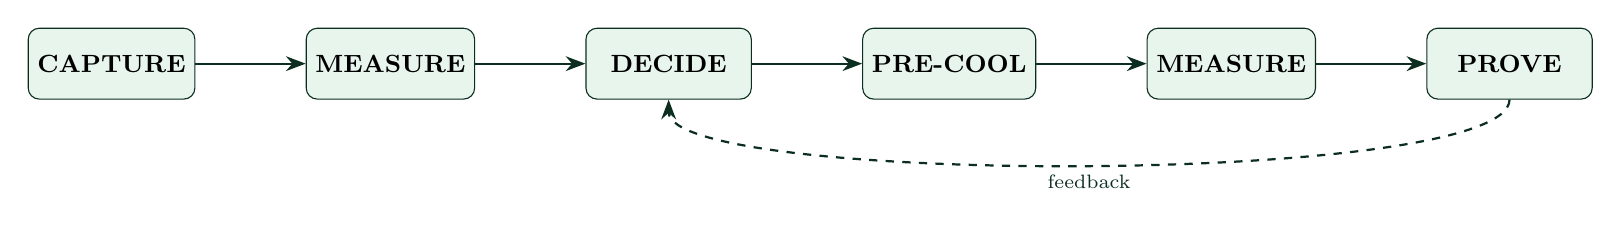
\begin{tikzpicture}[
    node distance=1.4cm,
    box/.style={rectangle, draw=climoragreen, fill=climoralight, rounded corners, minimum width=2.1cm, minimum height=0.9cm, align=center, font=\small\bfseries},
    arr/.style={-{Stealth[length=2.5mm]}, thick, climoragreen}
]
\node[box] (c) {CAPTURE};
\node[box, right=of c] (m) {MEASURE};
\node[box, right=of m] (d) {DECIDE};
\node[box, right=of d] (p) {PRE-COOL};
\node[box, right=of p] (m2) {MEASURE};
\node[box, right=of m2] (pr) {PROVE};
\draw[arr] (c) -- (m);
\draw[arr] (m) -- (d);
\draw[arr] (d) -- (p);
\draw[arr] (p) -- (m2);
\draw[arr] (m2) -- (pr);
\draw[arr, dashed] (pr.south) .. controls +(0,-1.1) and +(0,-1.1) .. node[below, font=\scriptsize]{feedback} (d.south);
\end{tikzpicture}
\caption{CLIMORA's six-stage operating loop.}
\end{figure}

\begin{enumerate}
    \item \textbf{Capture} -- AC condensate is diverted into a collection tank via a T-junction, while the original drain remains permanently open (Section~\ref{sec:architecture}).
    \item \textbf{Measure} -- Sensors continuously read climate, AC electrical load, condensate mass, and condenser temperature.
    \item \textbf{Decide} -- A deterministic rule engine evaluates whether pre-cooling is currently worthwhile (Section~\ref{sec:control}).
    \item \textbf{Pre-cool} -- If justified, an ultrasonic atomizer mists the condenser inlet.
    \item \textbf{Measure} -- The system logs AC power, condenser thermal response, and water consumption throughout.
    \item \textbf{Prove} -- Net energy saved, water balance, and comfort compliance are computed and reported (Section~\ref{sec:energy}).
\end{enumerate}

% =====================================================================
\section{What Is Novel}
\label{sec:novelty}
% =====================================================================

\textbf{Existing mechanism} \validated: Condensate-assisted adiabatic condenser pre-cooling is demonstrated in peer-reviewed literature -- specifically Pichandi et al.\ (2025), tested on a 1-ton AC in Chennai (Section~\ref{sec:literature}). CLIMORA does not claim to have invented this physical mechanism.

\textbf{CLIMORA's novelty:} A demand-aware control and measurement layer that decides, in real time, whether pre-cooling should operate, based on:
\begin{itemize}
    \item Water availability (measured condensate mass, not assumed supply)
    \item Climate conditions (wet-bulb depression -- real evaporative potential, right now)
    \item AC electrical load (is the compressor working hard enough to benefit?)
    \item Condenser thermal response (is misting actually helping, or just wetting the coil?)
    \item Occupant comfort (is the indoor environment within its configured boundary?)
    \item System health (are all relevant sensors functioning?)
\end{itemize}

\begin{keyidea}
The contribution is not ``we spray condensate on a condenser.'' It is ``we built the decision layer that determines when spraying condensate is actually worth it'' -- and we measure our own result rather than citing someone else's.
\end{keyidea}

CLIMORA must never be described, internally or externally, as simply ``an AC water-saving system'' or ``a condensate recycling gadget.'' The correct framing is always the full loop in Section~\ref{sec:concept}.

% =====================================================================
\section{System Architecture}
\label{sec:architecture}
% =====================================================================

\begin{figure}[h!]
\centering
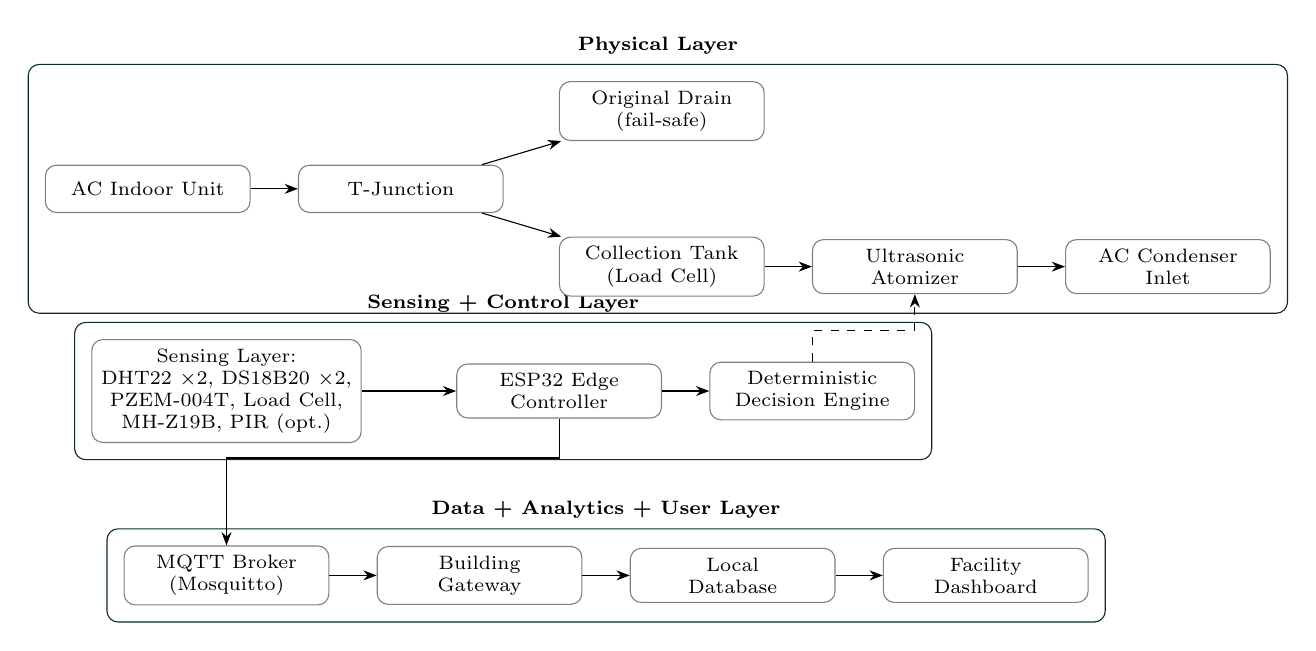
\begin{tikzpicture}[
    node distance=0.5cm and 0.6cm,
    every node/.style={font=\scriptsize},
    layer/.style={rectangle, draw=climoragreen, rounded corners, inner sep=6pt},
    comp/.style={rectangle, draw=black!50, fill=white, rounded corners, minimum width=2.6cm, minimum height=0.6cm, align=center}
]
% Physical layer
\node[comp] (ac) {AC Indoor Unit};
\node[comp, right=of ac] (tj) {T-Junction};
\node[comp, above right=0.3cm and 0.7cm of tj] (od) {Original Drain\\(fail-safe)};
\node[comp, below right=0.3cm and 0.7cm of tj] (tank) {Collection Tank\\(Load Cell)};
\node[comp, right=of tank] (atom) {Ultrasonic\\Atomizer};
\node[comp, right=of atom] (cond) {AC Condenser\\Inlet};

\draw[-{Stealth}] (ac) -- (tj);
\draw[-{Stealth}] (tj) -- (od);
\draw[-{Stealth}] (tj) -- (tank);
\draw[-{Stealth}] (tank) -- (atom);
\draw[-{Stealth}] (atom) -- (cond);

\begin{scope}[on background layer]
\node[layer, fit=(ac)(tj)(od)(tank)(atom)(cond), label=above:{\bfseries Physical Layer}] {};
\end{scope}

% Sensing + control below
\node[comp, below=1.6cm of ac, xshift=1cm] (sens) {Sensing Layer:\\DHT22 $\times$2, DS18B20 $\times$2,\\PZEM-004T, Load Cell,\\MH-Z19B, PIR (opt.)};
\node[comp, right=1.2cm of sens] (esp) {ESP32 Edge\\Controller};
\node[comp, right=of esp] (decide) {Deterministic\\Decision Engine};

\draw[-{Stealth}] (sens) -- (esp);
\draw[-{Stealth}] (esp) -- (decide);
\draw[-{Stealth}, dashed] (decide.north) -- ++(0,0.4) -| (atom.south);

\begin{scope}[on background layer]
\node[layer, fit=(sens)(esp)(decide), label=above:{\bfseries Sensing + Control Layer}] {};
\end{scope}

% Data + analytics layer
\node[comp, below=1.3cm of sens] (mqtt) {MQTT Broker\\(Mosquitto)};
\node[comp, right=of mqtt] (gw) {Building\\Gateway};
\node[comp, right=of gw] (db) {Local\\Database};
\node[comp, right=of db] (dash) {Facility\\Dashboard};

\draw[-{Stealth}] (esp.south) -- ++(0,-0.5) -| (mqtt.north);
\draw[-{Stealth}] (mqtt) -- (gw);
\draw[-{Stealth}] (gw) -- (db);
\draw[-{Stealth}] (db) -- (dash);

\begin{scope}[on background layer]
\node[layer, fit=(mqtt)(gw)(db)(dash), label=above:{\bfseries Data + Analytics + User Layer}] {};
\end{scope}

\end{tikzpicture}
\caption{CLIMORA system architecture: physical water/air path, sensing and control, and the data/analytics layer.}
\end{figure}

\begin{table}[h!]
\centering
\caption{Architecture layer summary}
\begin{tabular}{p{2.6cm}p{5.5cm}p{5.5cm}}
\toprule
\textbf{Layer} & \textbf{Components} & \textbf{Role} \\
\midrule
Physical & T-junction, tank, atomizer, condenser & The actual water and air path \\
Sensing & DHT22, DS18B20, PZEM-004T, load cell, MH-Z19B, optional PIR & All measurement inputs \\
Control & ESP32, deterministic decision engine & Local, safety-critical decision-making \\
Data & MQTT/Mosquitto, local database, gateway & Telemetry transport and storage \\
Analytics \& User & Dashboard, mock API/BMS interface & Human-facing visibility and (future) BMS integration \simulation\future \\
\bottomrule
\end{tabular}
\end{table}

\subsection{End-to-End Operating Flow}
\begin{enumerate}
    \item AC operates normally, cooling the space.
    \item Condensate forms at the indoor unit's evaporator coil.
    \item Condensate is diverted through a T-junction; the original drain path remains open at all times.
    \item The load cell measures the mass of water captured in the collection tank over time.
    \item Sensors continuously measure indoor/outdoor temperature and humidity, AC electrical load, and condenser-side temperature.
    \item The decision engine evaluates whether all activation conditions are satisfied (Section~\ref{sec:control}).
    \item If satisfied, the ultrasonic atomizer mists the condenser inlet; duty cycle is set according to available water.
    \item Condenser thermal response is monitored continuously -- if the coil is not responding, misting stops (the ``do-no-harm'' guard).
    \item The system reverts to HOLD whenever any activation condition is no longer satisfied.
    \item Energy, water balance, and comfort/IAQ status are logged throughout.
    \item The dashboard reports live status and aggregated performance to the facility manager.
\end{enumerate}

% =====================================================================
\section{Hardware \& Bill of Materials}
\label{sec:bom}
% =====================================================================

\begin{limitation}
Estimated prototype cost: \textbf{\textrupee7{,}000--\textrupee8{,}500}, depending on component sourcing. This is the current figure for prototype cost -- any older figure (\textrupee6{,}270 or \textrupee6{,}329) appearing elsewhere is stale and superseded, following a verified MH-Z19B price correction.
\end{limitation}

\begin{longtable}{p{4.3cm}p{5.3cm}p{1.6cm}p{2.3cm}}
\caption{Prototype Bill of Materials} \\
\toprule
\textbf{Component} & \textbf{Purpose} & \textbf{Cost (INR)} & \textbf{Status} \\
\midrule
\endfirsthead
\toprule
\textbf{Component} & \textbf{Purpose} & \textbf{Cost (INR)} & \textbf{Status} \\
\midrule
\endhead
ESP32 DevKit (WROOM-32) & Edge controller, WiFi, hosts dashboard interface & 450 & \prototype \\
PZEM-004T AC energy meter & Real power (W), power factor, cumulative kWh & 650 & \prototype \\
MH-Z19B NDIR CO\textsubscript{2} sensor & CO\textsubscript{2} ppm -- occupant air-quality proxy & 2{,}700--3{,}000 & \prototype \\
DHT22 $\times$2 & Indoor + outdoor air temperature/RH & 700 & \prototype \\
DS18B20 waterproof $\times$2 & Condenser-side inlet-air temp.\ + coil/surface temp.\ & 200 & \prototype \\
Load cell (1\,kg) + HX711 amplifier & Tank mass over time $\rightarrow$ condensate capture rate & 270 & \prototype \\
Ultrasonic atomizer + driver (24V, 36mm) & Delivers fine mist to condenser inlet & 359 & \prototype \tobevalidated \\
5V relay module & Switches atomizer on/off from ESP32 & 150 & \prototype \\
Water level float switch & High/low level protection & $\sim$150 & \prototype \\
Reservoir, overflow T-junction, tubing, enclosure, wiring, 12V PSU & Physical build and safe water-path hardware & $\sim$1{,}600 & \prototype \\
PIR motion sensor (HC-SR501) -- optional & Occupancy context (occupied/unoccupied) & $\sim$50--80 & \prototype \\
\bottomrule
\end{longtable}

\begin{table}[h!]
\centering
\caption{Components explicitly removed from the BOM, with reasons}
\begin{tabular}{p{3.3cm}p{10cm}}
\toprule
\textbf{Removed component} & \textbf{Reason} \\
\midrule
YF-S201 flow sensor & Usable range starts $\sim$1\,L/min; expected condensate flow is $\sim$0.01--0.015\,L/min -- 65--100$\times$ below sensor floor. Replaced by load cell + HX711 mass measurement. \\
Generic 12V pump + nozzles & Flow-mismatched to condensate rate; would pool or run the tank dry. Replaced by an ultrasonic atomizer. \\
Peltier module (TEC1-12706) & Low COP ($\sim$0.3--0.5 air-cooled); irrelevant to the actual water source (condensate, not ambient-air condensation). \\
MQ-135 gas sensor & Broad metal-oxide sensor, not selective for CO\textsubscript{2} (ppm). Replaced by MH-Z19B (NDIR). \\
ACS712 current sensor & Measures current only; cannot establish true kWh without voltage and power factor. Replaced by PZEM-004T. \\
\bottomrule
\end{tabular}
\end{table}

\begin{limitation}
Do not state a specific mL/h or L/h figure for the atomizer in any submission material. If asked: ``The selected atomizer's exact output will be experimentally characterized against the measured condensate capture rate before deployment.''
\end{limitation}

% =====================================================================
\section{Software Architecture}
% =====================================================================

\textbf{Prototype software (hackathon stage):}
\begin{itemize}
    \item \textbf{ESP32 firmware} -- reads all sensors, runs the deterministic decision engine locally, drives the atomizer relay, publishes telemetry.
    \item \textbf{MQTT (Mosquitto, self-hosted)} -- publishes to topics such as \texttt{building/ac07/energy}, \texttt{building/ac07/comfort}, \texttt{building/ac07/status}, \texttt{building/ac07/mode}; subscribes to \texttt{building/commands/ac07/demand-response} for simulated grid events.
    \item \textbf{Local dashboard} -- a lightweight web interface (ESP32-hosted or a simple Flask/Node-RED layer).
    \item \textbf{Mock REST API}:
    \begin{verbatim}
GET  /building/energy
GET  /hvac/status
GET  /hvac/{unit_id}/history
POST /demand-response
POST /setpoint   (logged only -- does not modify the AC)
    \end{verbatim}
\end{itemize}

\begin{simbox}
The mock MQTT/REST layer is a believable, buildable demo pattern -- it is explicitly not a claim of commercial BMS or BACnet certification. \future: multiple AC nodes aggregated through a building gateway into a proper timeseries database and analytics engine, with authenticated API access for a real BMS.
\end{simbox}

% =====================================================================
\section{Control \& Decision Engine}
\label{sec:control}
% =====================================================================

\textbf{Design philosophy:} CLIMORA is deterministic at the safety/control layer. Any prediction or AI component (Section~\ref{sec:ai}) may recommend; it never has direct actuation authority. A transparent, calibratable rule is both easier to validate and safer for a system with a physical actuator in occupied space.

\textbf{Core decision logic:}
\begin{verbatim}
IF   wet_bulb_depression > T1          (real evaporative cooling potential exists)
AND  condenser_air_inlet_temp > T2     (condenser is actually thermally stressed)
AND  ac_load > T3                      (compressor working hard enough to benefit)
AND  tank_mass > minimum_reserve       (sufficient captured condensate available)
AND  recent_condensate_capture_rate is sufficient  (trailing-window, not instantaneous)
AND  indoor_temp/RH within configured comfort boundary
AND  all relevant sensors report healthy
THEN ACTIVATE pre-cooling (duty cycle set according to available water)
ELSE HOLD (do not mist; conserve water)
\end{verbatim}

\textbf{Condenser ``do-no-harm'' guard} (runs continuously while pre-cooling is active):
\begin{verbatim}
WHILE pre-cooling ACTIVE:
    MONITOR condenser_coil_surface_temp
    IF coil_surface_temp is NOT decreasing after a short check interval:
        STOP misting (possible coil flooding/filming) and flag for review
    ELSE:
        continue, subject to a maximum duty cycle (calibrated experimentally)
\end{verbatim}

\tobevalidated: Threshold values ($T_1$, $T_2$, $T_3$, minimum reserve, comfort boundary) are calibration parameters established experimentally during prototype testing -- not hard-coded assumptions.

\textbf{HOLD conditions} (CLIMORA deliberately does \emph{not} run pre-cooling when):
\begin{itemize}[nosep]
    \item Water availability is insufficient
    \item AC electrical load is too low to meaningfully benefit
    \item Evaporative potential is poor (wet-bulb depression below threshold)
    \item The condenser is not actually responding to misting (do-no-harm guard)
    \item The comfort boundary would be exceeded
    \item Any relevant sensor has failed (fail-safe default)
\end{itemize}

\begin{keyidea}
This HOLD list is itself a differentiator: CLIMORA is not blindly trying to save energy -- it is actively deciding when \emph{not} to act.
\end{keyidea}

% =====================================================================
\section{AI / Predictive Layer}
\label{sec:ai}
% =====================================================================

AI in CLIMORA is explicitly advisory, never a direct controller of the physical actuator.

\textbf{What AI/prediction does} \future:
\begin{itemize}
    \item \textbf{Condensate generation prediction} -- a lightweight regression (indoor/outdoor RH and temperature, AC load, historical capture-rate log) estimating expected condensate availability over the next $\sim$30 minutes.
    \item \textbf{Adaptive thresholds} -- periodically recalibrating $T_1$/$T_2$/$T_3$ from logged outcomes, compared against fixed-threshold performance as an explicit A/B measurement.
    \item \textbf{Anomaly detection / predictive maintenance} -- flagging declining atomizer output or condenser thermal-response trends.
\end{itemize}

\begin{figure}[h!]
\centering
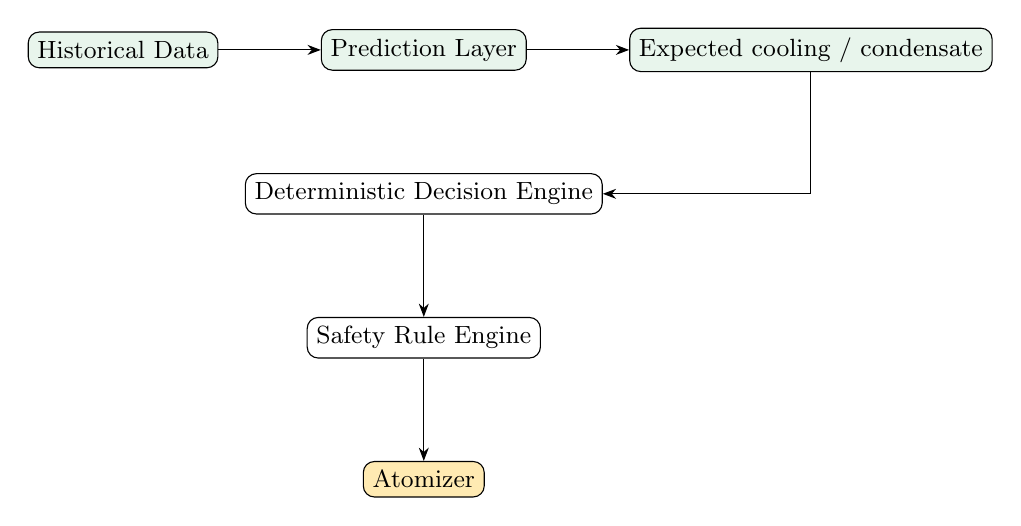
\begin{tikzpicture}[node distance=1.3cm, every node/.style={font=\small}]
\node[rectangle, draw, rounded corners, fill=climoralight] (hist) {Historical Data};
\node[rectangle, draw, rounded corners, fill=climoralight, right=of hist] (pred) {Prediction Layer};
\node[rectangle, draw, rounded corners, fill=climoralight, right=of pred] (exp) {Expected cooling / condensate};
\node[rectangle, draw, rounded corners, fill=white, below=of pred] (engine) {Deterministic Decision Engine};
\node[rectangle, draw, rounded corners, fill=white, below=of engine] (safety) {Safety Rule Engine};
\node[rectangle, draw, rounded corners, fill=climoraamber!30, below=of safety] (act) {Atomizer};
\draw[-{Stealth}] (hist) -- (pred);
\draw[-{Stealth}] (pred) -- (exp);
\draw[-{Stealth}] (exp.south) |- (engine.east);
\draw[-{Stealth}] (engine) -- (safety);
\draw[-{Stealth}] (safety) -- (act);
\end{tikzpicture}
\caption{AI recommends; the deterministic safety engine protects the building.}
\end{figure}

\textbf{What AI does NOT control:} it does not directly switch the atomizer on/off, does not modify the AC setpoint, and is never described as ``autonomously optimizing everything.''

\begin{limitation}
``Prediction/AI recommends; the deterministic safety engine protects the building.'' This framing is deliberate and must be used consistently in any judge-facing explanation.
\end{limitation}

% =====================================================================
\section{Occupant Experience \& IAQ}
\label{sec:iaq}
% =====================================================================

\begin{table}[h!]
\centering
\caption{Occupant-experience sensing}
\begin{tabular}{lll}
\toprule
\textbf{Parameter} & \textbf{Sensor} & \textbf{Role} \\
\midrule
Indoor temperature & DHT22 & Comfort monitoring \\
Indoor relative humidity & DHT22 & Comfort monitoring \\
CO\textsubscript{2} concentration (ppm) & MH-Z19B (NDIR) & Air-quality proxy \\
\bottomrule
\end{tabular}
\end{table}

\textbf{Comfort boundary:} a configurable band (e.g.\ 24--26$^\circ$C as a building-policy example, not a universal standard). If monitored indoor temperature/RH moves outside this boundary, pre-cooling is \textbf{suspended} -- stated as ``suspended if exceeded,'' not ``guaranteed,'' since CLIMORA does not control the AC setpoint or compressor directly.

\textbf{IAQ alert logic:} \texttt{IF CO2 > threshold THEN raise IAQ alert on dashboard}. CLIMORA never reduces ventilation to save energy and does not claim to manage ventilation -- the alert is informational.

\begin{limitation}
Energy efficiency is pursued only within defined occupant-comfort and safety boundaries. CLIMORA must never be framed as ``save energy first, comfort second.''
\end{limitation}

% =====================================================================
\section{Energy Measurement \& Validation}
\label{sec:energy}
% =====================================================================

\textbf{Net Energy Saving} (the only energy-saving formula CLIMORA uses):
\begin{align}
\text{Net Energy Saving} &= E_{AC,\text{baseline}} - \left(E_{AC,\text{intervention}} + E_{\text{auxiliary}}\right) \\
\text{Net Saving (\%)} &= \frac{E_{AC,\text{baseline}} - \left(E_{AC,\text{intervention}} + E_{\text{auxiliary}}\right)}{E_{AC,\text{baseline}}} \times 100
\end{align}
where $E_{\text{auxiliary}}$ includes the atomizer's electricity and relay/control electronics during the intervention window.

\textbf{Testing methodology -- ``IPMVP-inspired short-duration comparative testing''} (explicitly not a full IPMVP certification):
\begin{itemize}
    \item Same AC unit, same setpoint, same room, doors/windows closed, same fan setting.
    \item Four back-to-back 45--60 minute cycles: Baseline $\rightarrow$ Intervention $\rightarrow$ Baseline $\rightarrow$ Intervention, same test day.
    \item Continuous logging: AC electrical energy, auxiliary energy, indoor/outdoor temp/RH, condensate capture, water usage, condenser thermal response.
    \item Repeated across at least two separate days/times of day.
\end{itemize}

\textbf{Experimental validity tolerance:} a result is counted as valid only if indoor temperature/RH during the intervention run stayed within $\pm1^\circ$C and $\pm5\%$ RH of the baseline run's band -- a test-validity rule, not a comfort standard.

\begin{table}[h!]
\centering
\caption{Three-tier evidence separation}
\begin{tabular}{p{3.2cm}p{3.2cm}p{6cm}}
\toprule
\textbf{Tier} & \textbf{Value} & \textbf{Status} \\
\midrule
Literature result & $\sim$39.2\% & \validated\ -- belongs to the cited study, not CLIMORA \\
CLIMORA target & $\geq$5\% net reduction & \design\ -- a conservative, stated target \\
CLIMORA measured result & Not yet available & \tobevalidated \\
\bottomrule
\end{tabular}
\end{table}

\begin{limitation}
CLIMORA has not yet experimentally validated its own energy savings. Do not state or imply ``CLIMORA saves 39.2\% energy'' anywhere.
\end{limitation}

\textbf{Scale-up formula:}
\begin{equation}
\text{Annual Energy Saving} = \text{Measured Net Saving Rate (kWh/h)} \times \text{Annual Operating Hours} \times \text{Number of AC units}
\end{equation}

% =====================================================================
\section{Water Accounting}
% =====================================================================

\textbf{Capture measurement:} condensate \emph{captured} (not total AC condensate \emph{generated}) is measured as the tank's mass increase over time via the load cell. The T-junction allows excess condensate to bypass directly to the original drain, which the load cell cannot see -- ``captured'' is the physically accurate and operationally relevant term.

\textbf{Water balance} (kept in mass/grams throughout):
\begin{equation}
M_{\text{final}} = M_{\text{initial}} + M_{\text{captured}} - M_{\text{used}} - M_{\text{drained}}
\end{equation}

\begin{itemize}[nosep]
    \item $M_{\text{initial}}$ -- tank mass at the start of the measurement window
    \item $M_{\text{captured}}$ -- condensate captured during the window (measured)
    \item $M_{\text{used}}$ -- water consumed by the atomizer during pre-cooling
    \item $M_{\text{drained}}$ -- water discharged through overflow/original drain
\end{itemize}

\begin{equation}
\text{Water efficiency} = \frac{\text{grams reused}}{\text{kWh net saved}}
\end{equation}

% =====================================================================
\section{Grid / Demand Response}
\label{sec:grid}
% =====================================================================

\begin{simbox}
Grid integration is a simulated, prototype-stage concept. CLIMORA does not claim live DISCOM or utility integration. This is explicitly labeled an \textbf{OpenADR-inspired demand-response simulation}, consistent with the hackathon's problem statement, which qualifies this outcome with ``where DISCOM programmes allow.''
\end{simbox}

\begin{table}[h!]
\centering
\caption{Operating modes}
\begin{tabular}{lp{9cm}}
\toprule
\textbf{Mode} & \textbf{Behavior} \\
\midrule
Normal & Comfort priority; no forced load reduction \\
Efficiency & Pre-cooling active per Section~\ref{sec:control}, maximizing net saving within constraints \\
Peak/Grid & Triggered by simulated demand-response signal; increases pre-cooling duty \emph{if water allows}; never modifies the AC setpoint \\
\bottomrule
\end{tabular}
\end{table}

\textbf{Simulated event lifecycle} (OpenADR-inspired, not protocol-compliant):
\begin{enumerate}[nosep]
    \item Event signal -- mock ``utility'' script/button posts a DR event (id, start time, duration)
    \item Event received -- CLIMORA logs baseline kW just before response begins
    \item Load response -- Peak/Grid Mode activates (increased pre-cooling duty, no setpoint change)
    \item Reduction calculated (formula below)
    \item Event end + report -- result published via MQTT/REST
\end{enumerate}

\begin{equation}
\text{Peak Load Reduction (kW)} = P_{\text{baseline}} - P_{\text{grid mode}}, \qquad
\text{Load Reduction (\%)} = \frac{P_{\text{baseline}} - P_{\text{grid mode}}}{P_{\text{baseline}}} \times 100
\end{equation}

% =====================================================================
\section{Fault Detection \& Fail-Safe Design}
\label{sec:failsafe}
% =====================================================================

\textbf{The single most important safety property:} the AC's original condensate drain is always available, under every failure mode.

\begin{figure}[h!]
\centering
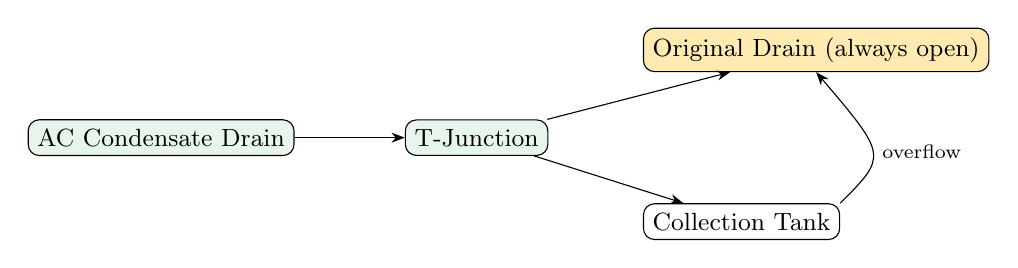
\begin{tikzpicture}[node distance=1.4cm, every node/.style={font=\small}]
\node[rectangle, draw, rounded corners, fill=climoralight] (ac) {AC Condensate Drain};
\node[rectangle, draw, rounded corners, fill=climoralight, right=of ac] (tj) {T-Junction};
\node[rectangle, draw, rounded corners, fill=climoraamber!30, above right=0.6cm and 1.2cm of tj] (od) {Original Drain (always open)};
\node[rectangle, draw, rounded corners, fill=white, below right=0.6cm and 1.2cm of tj] (tank) {Collection Tank};
\draw[-{Stealth}] (ac) -- (tj);
\draw[-{Stealth}] (tj) -- (od);
\draw[-{Stealth}] (tj) -- (tank);
\draw[-{Stealth}] (tank.north east) .. controls +(0.6,0.6) .. node[right, font=\scriptsize]{overflow} (od.south);
\end{tikzpicture}
\caption{The collection tank is a branch off the drain path, never a replacement for it.}
\end{figure}

\begin{longtable}{p{2.8cm}p{3.6cm}p{4.2cm}p{3.5cm}}
\caption{Failure-mode matrix} \\
\toprule
\textbf{Failure} & \textbf{Detection} & \textbf{Response} & \textbf{Safety consequence} \\
\midrule
\endfirsthead
\toprule
\textbf{Failure} & \textbf{Detection} & \textbf{Response} & \textbf{Safety consequence} \\
\midrule
\endhead
Tank full & Water level / overflow geometry & Gravity overflow to original drain & None -- drainage unaffected \\
Tank empty / low water & Float switch & Atomizer OFF & None -- pre-cooling simply doesn't run \\
Atomizer blocked/fault & Commanded ON + mass not decreasing & Fault alert raised & Pre-cooling disabled until resolved \\
Sensor failure (any) & Expected-value/health check & Disable pre-cooling, default to HOLD & Fail-safe default, not fail-open \\
Network/WiFi lost & Connectivity check & Local decision engine continues safely & No loss of safety-critical function \\
Comfort boundary exceeded & Indoor DHT22 reading & Pre-cooling suspended & Comfort protected \\
Condenser not responding & Coil-surface temp trend & Stop misting, flag for review & Prevents coil flooding/filming \\
Power failure & -- & Passive revert to original-drain-only & No active component required \\
Controller failure & -- & Original drain remains fully functional & Architecture-level guarantee \\
\bottomrule
\end{longtable}

% =====================================================================
\section{Physical Installation \& Retrofit}
% =====================================================================

\begin{enumerate}
    \item Identify the AC's condensate drain line.
    \item Install a T-junction with a gravity-fed overflow bypass to the original drain.
    \item Mount a covered reservoir with the load cell and level float switch.
    \item Install the ultrasonic atomizer near the condenser inlet.
    \item Install DHT22 $\times2$, DS18B20 $\times2$, MH-Z19B, PZEM-004T, optional PIR, and the ESP32 controller with wiring.
    \item Calibrate decision-engine thresholds and the comfort band.
    \item Run a baseline measurement period before activating pre-cooling logic.
\end{enumerate}

\textbf{No invasive modification of the refrigeration circuit is required.} Maintenance: a closed, covered reservoir, an explicit no-potable-use label, and a manual drain/cleaning procedure (no automated flush exists in the current BOM). An optional inline sediment filter before the atomizer reduces clogging risk.

% =====================================================================
\section{Testing Plan}
% =====================================================================

\textbf{Prototype validation (current scope):}
\begin{itemize}[nosep]
    \item Controlled A/B/A/B comparative testing (Section~\ref{sec:energy}).
    \item Variables logged: AC/auxiliary energy, indoor/outdoor temp/RH, condensate capture, water usage, condenser thermal response.
    \item Acceptance criterion: within $\pm1^\circ$C, $\pm5\%$ RH of baseline.
    \item Repetition: at least two separate days/times of day.
\end{itemize}

\textbf{Future field validation} \future:
\begin{itemize}[nosep]
    \item Multi-unit, multi-building testing across different climate zones.
    \item Longer-duration fouling/scaling studies on the atomizer and condenser.
    \item Real building-manager usability testing of the dashboard and alert workflow.
\end{itemize}

% =====================================================================
\section{Economics \& Scalability}
% =====================================================================

\textbf{Baseline assumptions} (commonly-cited benchmarks, not CLIMORA-specific measurements): a representative 1.5--2 ton commercial split/ducted AC draws $\sim$1.75\,kW average; commercial operation $\sim$9\,hrs/day, $\sim$200 cooling days/year.

\begin{align}
\text{Annual baseline energy per AC} &= 1.75\,\text{kW} \times 9\,\text{hrs} \times 200\,\text{days} = 3{,}150\,\text{kWh/year} \\
\text{Annual cost per AC (at \textrupee9/kWh)} &= 3{,}150 \times 9 = \text{\textrupee}28{,}350/\text{year}
\end{align}

\begin{table}[h!]
\centering
\caption{Illustrative savings and payback (target range, not yet measured)}
\begin{tabular}{lcccc}
\toprule
\textbf{Saving \%} & \textbf{kWh/yr saved} & \textbf{\textrupee/yr saved} & \textbf{Payback @\textrupee4k} & \textbf{Payback @\textrupee8k} \\
\midrule
5\% (conservative) & 157.5 & 1{,}418 & 2.8 yr & 5.6 yr \\
10\% (midpoint) & 315 & 2{,}835 & 1.4 yr & 2.8 yr \\
15\% (literature-adjacent) & 472.5 & 4{,}253 & 0.9 yr & 1.9 yr \\
\bottomrule
\end{tabular}
\end{table}

\begin{table}[h!]
\centering
\caption{Scaled to building types (linear scaling; per-unit payback identical by construction)}
\begin{tabular}{lcccc}
\toprule
\textbf{Building type} & \textbf{AC units} & \textbf{Investment} & \textbf{Annual savings @10\%} & \textbf{Payback} \\
\midrule
Small office & 10 & \textrupee40,000--80,000 & \textrupee28,350 & 1.4--2.8 yr \\
Mid-size hotel & 50 & \textrupee2--4 lakh & \textrupee1,41,750 & 1.4--2.8 yr \\
Large commercial & 100 & \textrupee4--8 lakh & \textrupee2,83,500 & 1.4--2.8 yr \\
\bottomrule
\end{tabular}
\end{table}

\begin{limitation}
No guaranteed payback period is claimed. All figures above are illustrative, built on stated assumptions, pending real per-AC measured data.
\end{limitation}

One AC node's design is unchanged whether deployed singly or at building scale -- only the aggregation layer (gateway, database, analytics) is added.

% =====================================================================
\section{Sustainability \& Impact}
% =====================================================================

\textbf{Baseline (no system installed):} 0\,g condensate reused, 0\,kWh net saved, 100\% condensate discharged to drain.

\textbf{Intervention} (values measured during prototype validation):
\begin{align}
N\,\text{kg CO}_2\text{e avoided} &= Z\,\text{kWh} \times 0.705\,\text{kgCO}_2\text{/kWh}
\end{align}

\textbf{Emission factor source:} CEA CO\textsubscript{2} Baseline Database for the Indian Power Sector, User Guide Version 22.0 (August 2026), Combined Margin emission factor including cross-border transfers, \textbf{FY 2025-26 = 0.705\,kgCO\textsubscript{2}/kWh}. This factor falls each year as the grid decarbonizes (0.757 FY23-24 $\rightarrow$ 0.736 FY24-25 $\rightarrow$ 0.705 FY25-26) -- re-verify against the current CEA database version before final submission.

\begin{equation}
\text{\% condensate diverted from drain} = \frac{Y}{X} \times 100, \qquad
\text{Water efficiency} = \frac{Y\,\text{grams reused}}{Z\,\text{kWh net saved}}
\end{equation}

% =====================================================================
\section{Dashboard / User Experience}
% =====================================================================

\textbf{Facility-manager-facing dashboard fields:} current kW, cumulative kWh, net kWh saved, \textrupee\ saved, CO\textsubscript{2}e avoided, condensate captured, condensate reused, comfort state, IAQ state, grid/demand-response state, fault alerts, system health score.

\begin{quote}
\small
\texttt{ALERT: "AC-07 efficiency declining" -> "Possible condenser fouling detected"} \\
\texttt{-> "Recommended action: inspect condenser coil."}
\end{quote}

This converts raw sensor data and fault logic into genuinely actionable visibility -- directly answering the hackathon's requirement for ``clear, actionable visibility into energy use, equipment performance and occupancy patterns.''

% =====================================================================
\section{Metrics \& KPIs}
% =====================================================================

\begin{longtable}{p{3.2cm}p{5cm}p{5.8cm}}
\caption{Key performance indicators} \\
\toprule
\textbf{KPI} & \textbf{Formula / Definition} & \textbf{Why it matters} \\
\midrule
\endfirsthead
\toprule
\textbf{KPI} & \textbf{Formula / Definition} & \textbf{Why it matters} \\
\midrule
\endhead
Net Energy Saving & $E_{AC,base} - (E_{AC,int} + E_{aux})$ & The only honest energy-saving number \\
Net Saving \% & Net Energy Saving $/ E_{AC,base} \times 100$ & Comparable headline metric \\
Peak Load Reduction & $P_{base} - P_{grid}$ & Demonstrates demand-response capability \\
Condensate Captured & Load-cell mass increase & Water-resource accounting \\
Condensate Reused & Mass delta during atomizer-ON & Measures actual utilization \\
Water Utilization & Reused / Captured $\times 100$ & Efficiency of water usage \\
Comfort Compliance & \% time within comfort band & Validates comfort-as-constraint \\
IAQ Alerts & Count of CO\textsubscript{2}-threshold breaches & Occupant air-quality tracking \\
System Uptime & \% time controller/sensors healthy & Reliability tracking \\
Fault Detections & Count of alerts raised & Maintenance visibility \\
CO\textsubscript{2}e Avoided & Net kWh $\times$ 0.705 & Sustainability reporting \\
\textrupee\ Savings & Net kWh $\times$ tariff & Economic reporting \\
\bottomrule
\end{longtable}

% =====================================================================
\section{Literature \& Evidence}
\label{sec:literature}
% =====================================================================

\begin{table}[h!]
\centering
\small
\begin{tabular}{p{3.4cm}p{5cm}p{4cm}}
\toprule
\textbf{Source} & \textbf{What it demonstrates} & \textbf{CLIMORA's difference} \\
\midrule
Pichandi et al.\ (2025)~\cite{pichandi2025} & Condensate-assisted adiabatic pre-cooling, 1-ton AC, Chennai. Per-configuration water coverage: EC-pad $\sim$38\%, mist-only $\sim$50.7\%, hybrid $\sim$95\%. Hybrid: $\sim$39.2\% energy savings, COP 2.8$\to$5.0. & Simpler single-mechanism design (atomizer only), adds a demand-matched decision layer, independently measures its own performance. \\
BEE/ECBC Users' Manual~\cite{beeecbc} & HVAC $\approx$40\% of commercial building energy in India. & Establishes problem scale. \\
BEE commercial-building assessments~\cite{beeassessment} & Cooling electricity $\sim$1.07--1.59 million kWh/building/year (Mumbai, Delhi, Bangalore, Hyderabad). & Context for building-scale baselines. \\
CEA CO\textsubscript{2} Baseline Database v22.0~\cite{ceadb} & Combined Margin factor, FY2025-26 = 0.705\,kgCO\textsubscript{2}/kWh. & Used for all CO\textsubscript{2}e calculations. \\
\bottomrule
\end{tabular}
\caption{Literature and evidence base}
\end{table}

\begin{limitation}
None of the literature results above are CLIMORA's own measured results. They establish plausibility and context; CLIMORA's own performance must be experimentally validated.
\end{limitation}

% =====================================================================
\section{Assumptions, Unknowns \& Validation Gaps}
\label{sec:gaps}
% =====================================================================

This section exists to be read, not hidden. Technical credibility comes from stating these plainly.

\begin{longtable}{p{6.5cm}p{7cm}}
\caption{Open validation items} \\
\toprule
\textbf{Item} & \textbf{Status} \\
\midrule
\endfirsthead
\toprule
\textbf{Item} & \textbf{Status} \\
\midrule
\endhead
CLIMORA's actual net energy-saving percentage & \tobevalidated\ -- not yet measured \\
Exact atomizer output (mL/h, wattage) & \tobevalidated\ -- candidate product identified, datasheet figure unconfirmed \\
Decision-engine thresholds ($T_1,T_2,T_3$, reserve, duty-cycle \%) & \tobevalidated\ -- calibration parameters, not yet established \\
India climate-zone applicability matrix & \design\ based on domain knowledge, not a live weather-dataset lookup \\
Long-term atomizer/condenser fouling behavior & \tobevalidated \\
Building-scale economics & \tobevalidated\ -- illustrative model, not field data \\
Grid/demand-response integration & \simulation\ -- OpenADR-inspired only \\
BMS/API integration & \simulation\ -- mock layer only \\
Field deployment maintenance procedures & \future \\
AC-type scalability beyond split/cassette units & \future\ -- phased roadmap \\
\bottomrule
\end{longtable}

% =====================================================================
\section{Prototype Roadmap}
% =====================================================================

\begin{table}[h!]
\centering
\begin{tabular}{p{1.6cm}p{8cm}p{2.2cm}}
\toprule
\textbf{Phase} & \textbf{Description} & \textbf{Status} \\
\midrule
1 & Bench validation -- sensor/actuator checks, decision logic without a live AC & \prototype \\
2 & Single AC prototype -- full physical integration & \prototype \\
3 & Controlled comparative testing -- A/B/A/B protocol & \prototype \\
4 & Multi-condition testing -- different times/weather & \prototype \\
5 & Building pilot -- multiple AC units, gateway aggregation & \future \\
6 & BMS/grid integration -- real API, live demand-response & \future \\
\bottomrule
\end{tabular}
\caption{Phased prototype roadmap}
\end{table}

\section{Future Roadmap}

Realistic extensions only -- deliberately bounded:
\begin{itemize}[nosep]
    \item Real BMS integration (beyond the current mock MQTT/REST layer)
    \item Smart thermostat / VRF controller integration
    \item Adaptive threshold prediction trained on accumulated field data
    \item Predictive maintenance indicators (equipment health scoring)
    \item Building-level multi-AC orchestration
    \item Real demand-response integration once DISCOM programmes support it
    \item AC-type phased expansion: split/cassette $\to$ packaged/ducted $\to$ centralized/VRF
\end{itemize}

This list should not keep growing -- new additions require the same evidence/validation discipline as Section~\ref{sec:gaps}.

% =====================================================================
\section{Team Explanation Cheat Sheet}
% =====================================================================

\subsection*{30-Second Explanation}
\textit{``Air conditioners waste the condensate water they produce. CLIMORA captures it and uses it to cool the AC's condenser when that's actually worthwhile -- based on climate, load, and how much water is available -- cutting electricity use without touching comfort.''}

\subsection*{60-Second Explanation}
\textit{``Every AC produces condensate water that's normally drained away. Spraying that water on the outdoor condenser as fine mist is a known way to improve AC efficiency -- a 2025 peer-reviewed study demonstrated it in Chennai. What's missing is intelligence: existing approaches don't ask whether using the water right now is actually worth it. CLIMORA measures AC electrical load, condenser temperature, climate conditions, and available condensate mass, and only activates misting when all of those indicate real benefit. It never compromises comfort -- pre-cooling is suspended if indoor conditions drift outside a configured boundary. We measure net energy savings, not gross, because we subtract the atomizer's own power draw. The whole retrofit costs about \textrupee7,000--8,500 and needs no modification to the AC's refrigeration circuit.''}

\subsection*{Ten Questions a Judge May Ask}

\begin{enumerate}
    \item \textbf{What is actually novel, if the physical mechanism already exists?} The demand-matched decision layer -- deciding \emph{when} reusing condensate is worthwhile.
    \item \textbf{Why condensate specifically?} Water the AC already produces and discards -- zero additional cost, close to distilled water.
    \item \textbf{Why not a standard flow sensor?} Expected flow ($\sim$0.01--0.015\,L/min) is far below a YF-S201's $\sim$1\,L/min floor; a load cell resolves gram-level changes instead.
    \item \textbf{Why ultrasonic atomization, not pump + nozzle?} Generic nozzles are flow-mismatched to the condensate supply; an atomizer matches the actual regime.
    \item \textbf{What happens if the tank is empty?} Float switch disables the atomizer; system holds, no harm.
    \item \textbf{What happens if the controller fails?} Original drain remains fully functional -- the tank is a branch, never a replacement.
    \item \textbf{How do you prove energy savings?} Controlled A/B/A/B testing, Net Energy Saving formula, only valid trials counted.
    \item \textbf{Does it affect comfort?} No -- comfort is a hard constraint; pre-cooling suspends on boundary violation.
    \item \textbf{Is AI actually controlling the AC?} No -- prediction only recommends; the deterministic safety engine has final authority.
    \item \textbf{What happens in dry weather or a mild climate?} The system evaluates wet-bulb depression, load, and water availability, defaulting to HOLD when conditions don't justify action.
\end{enumerate}

% =====================================================================
\section*{Acknowledgements}
% =====================================================================
\addcontentsline{toc}{section}{Acknowledgements}
This work is submitted to the Yuva Yodha Tech Hackathon 2026 (Smart Buildings track) by Team CLIMORA. We acknowledge the authors of the anchor research reference (Pichandi et al., 2025) whose experimental work established the physical plausibility of condensate-assisted adiabatic pre-cooling, and the Bureau of Energy Efficiency (BEE) and Central Electricity Authority (CEA) for the benchmark and emission-factor data cited throughout this report.

% =====================================================================
\bibliographystyle{plain}
\bibliography{references}

\end{document}
